\chapter{Introduction}

\section{Introduction to AJIT}

AJIT is an indigenous processor which has been designed at IIT Bombay and is currently in its second design and manufacturing iteration.
AJIT is based on the open SPARC-v8 ISA and is currently a 32-bit processor. The current design runs at 100 MHz and has been manufactured at
SCL, Chandigarh using the 180nm technological node.

\begin{figure}[H]
\centering
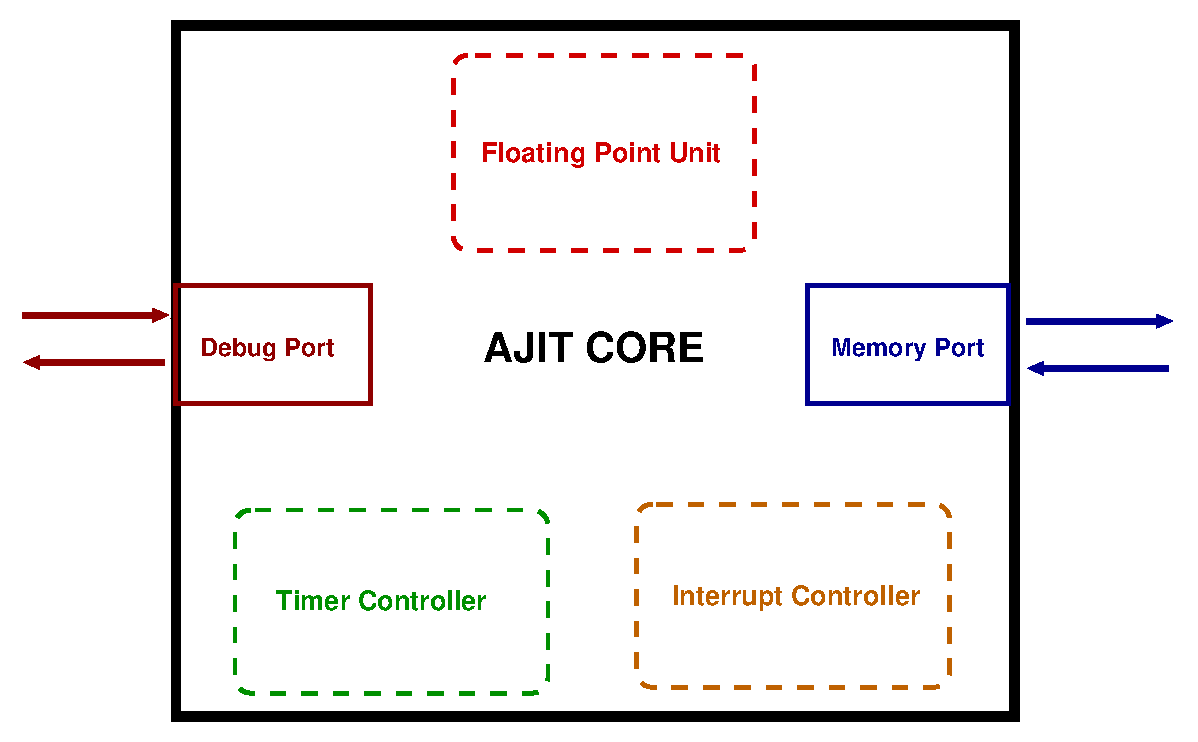
\includegraphics[scale=0.7]{eps_pdf_sources/ajit_fpga/AJIT/ajit_intro}
\caption{Overview of AJIT}
\end{figure}

\subsection{Support for AJIT}

AJIT has a functionally correct and verified C model which is used to verify new additions to the processor and user space
applications. AJIT also has a VHDL model which we incorporate into the later stages of this project and the same model later on loads
different programs ( before testing loading of an OS ) directly from the DRAM. 

\section{Introduction to the Project}

The main aim of this project is to provide an alternative to an earlier FPGA model designed around AJIT processor which had limited
on-board memory of 4MB and hence could borderline load a Linux system since the minimum memory requirement for a Linux operating system to
boot is around 4MB. The operating system thus loaded/booted had very limited kernel modules and userspace drivers to interface with hardware
elements.\\

This project is focussed at leveraging high DRAM storage capabilities and the high read and write speed of PCIe bus of the Xilinx VC709
board in order to make it capable to boot a heavily loaded embedded OS( quite possibly an RTOS ) with all the basic kernel modules and
userspace drivers to interface with hardware elements such as networking.\\

This process of booting an embedded OS on a FPGA platform is really advantageous as compared to booting OS on development boards based
around ASICs as we outline later. This project aims to integrate this FPGA system with a \verb|C++| based application to implement
a router system down the line.\\

We aim to incorporate soft core peripherals such as a Ethernet controller, USB controller etc to this FPGA system to ease the access to the
system through \verb|ssh| connections or through \verb|serial| connections. These kinds of easily integrable peripherals are expected to
make the development of custom applications really swift.\\

This project as we demonstrate later can also be used as a test-bed for HPC codecs development and testing. These peripherals can be
distributed along with the AJIT processor as part of its HPC peripheral library.
